\documentclass{article}

\usepackage[main,final]{neurips_2026}

\usepackage[utf8]{inputenc}
\usepackage[T1]{fontenc}
\usepackage{hyperref}
\usepackage{url}
\usepackage{booktabs}
\usepackage{amsfonts}
\usepackage{amsmath}
\usepackage{amssymb}
\usepackage{amsthm}
\usepackage{nicefrac}
\usepackage{microtype}
\usepackage{xcolor}
\usepackage{graphicx}
\usepackage{subcaption}
\usepackage{algorithm}
\usepackage{algorithmic}
\usepackage{multirow}
\usepackage{enumitem}
\usepackage{pifont}
\newcommand{\cmark}{\ding{51}}
\newcommand{\xmark}{\ding{55}}

\renewcommand{\qedsymbol}{$\blacksquare$}

\newtheorem{theorem}{Theorem}
\newtheorem{proposition}{Proposition}
\newtheorem{lemma}{Lemma}
\newtheorem{corollary}{Corollary}
\newtheorem{definition}{Definition}
\newtheorem{remark}{Remark}
\newtheorem{assumption}{Assumption}

\newcommand{\Xt}{\tilde{X}}
\newcommand{\Ft}{F_\theta}
\newcommand{\E}{\mathbb{E}}
\newcommand{\R}{\mathbb{R}}
\newcommand{\MI}{I}
\newcommand{\CE}{\mathrm{CE}}
\newcommand{\KL}{D_{\mathrm{KL}}}
\newcommand{\FMset}{\mathcal{F}}
\newcommand{\Estar}{E^{\star}}

\title{NeuroVeil-U: A Foundation-Model-Agnostic Privacy Filter for EEG\\via Ensemble Functional Surrogate Distillation}

\author{Anonymous}

\begin{document}
\maketitle

\begin{abstract}
Electroencephalogram (EEG) foundation models (FMs) are bottlenecked by the scarcity of public pretraining data because raw EEG signals carry biometric fingerprints that enable subject re-identification. Recent privacy filters mitigate this at the signal level but optimize a single utility surrogate---typically pure masked autoencoder (MAE) reconstruction---and are evaluated within-dataset, leaving two gaps: (i) cross-dataset transfer is weak and montage-sensitive, and (ii) downstream FMs that rely on vector-quantized (VQ) tokenization, autoregressive next-token prediction, or contrastive projection are not protected by an MSE-only filter. We propose \textbf{NeuroVeil-U}, a single bounded-perturbation filter that addresses both gaps. Three components are combined into one architecture: a \emph{channel-agnostic} LUNA-style generator with MNE standard-1005 coordinate embedding; an \emph{Ensemble Functional Surrogate} $\Estar$ distilled offline from a five-FM ensemble (BIOT, LaBraM, CBraMod, CodeBrain, REVE) that compresses the utility-preservation objective of four pretraining paradigms into one differentiable student; and a \emph{thirteen-head adversary suite} comprising four identity CNNs, five FM-representation probes, and a site-adversarial gradient-reversal head over 64 TUEG pseudo-sites (hospital~$\times$~year). At a 1{,}000-subject TUEG training scale on a single NVIDIA A40 GPU ($\sim\!95$ minutes of Phase-2 joint training), NeuroVeil-U simultaneously: (a) reduces same-dataset re-identification on TUEG val from $78.72\%$ to $25.94\%$ (\textbf{APG $\mathbf{67.10\%}$}, 338 subjects, retrained DeepCNN attacker, perturbation RMS $1.55$, mean channel correlation $0.60$); (b) delivers an $\mathbf{80.41\%}$ average zero-shot APG on two external datasets---TUSL (APG $72.48\%$, 19ch matched) and HMC (APG $\mathbf{88.33\%}$, 4-channel bipolar montage unseen during training); and (c) preserves linear-probe utility across all five foundation models on TUAB within $6\%$ of the unfiltered baseline simultaneously (average utility ratio \textbf{0.955}; per-FM: LaBraM $0.968$, CBraMod $0.964$, BIOT $0.954$, CodeBrain $0.946$, REVE $0.941$). An ablation confirms that moving from a light configuration to our V4-aligned training recipe lifts TUEG APG from $1.1\%$ to $67.1\%$ and the two-dataset cross-dataset APG from $3.4\%$ to $80.4\%$ at a $4.4$ percentage-point FM-utility cost, establishing the combined contribution of progressive perturbation, adversary refresh, and strong-privacy scheduling. All external-dataset comparisons use identical per-subject stratified retrained-attacker protocols. We release code, evaluation protocols, and all trained checkpoints.
\end{abstract}

%=============================================================
\section{Introduction}
\label{sec:intro}
%=============================================================

Electroencephalogram (EEG) foundation models (FMs) have recently achieved strong transfer across clinical tasks including seizure detection, sleep staging, pathology classification, and emotion recognition~\citep{labram,eegpt,cbramod,biot,reve}. Scaling the pretraining corpus beyond the ${\sim}25{,}000$ hours available to the strongest open models is blocked not by compute but by \emph{data}: hospitals hold vast unlabeled EEG recordings but are reluctant to share them because the raw signals carry biometric fingerprints that enable subject re-identification~\citep{eeg_biometric_survey,fallahi2026eeg_biometric,eeg_reidentification}.

Learned privacy filters that apply a bounded perturbation to the signal have emerged as the natural interface for data release~\citep{unlearnable_eeg_meng,adversarial_filter,wang2025idremovalnet}. A filter takes raw EEG $X$ and returns $\Xt = X + \delta\cdot\tanh(G_\theta(X))$ with an architecturally enforced $\ell_\infty$ bound, trained adversarially against a subject-identification attacker while preserving a surrogate utility signal such as masked autoencoder (MAE) reconstruction~\citep{mae}. However, two structural problems remain open.

\textbf{Problem A: cross-dataset transfer is weak.} A filter trained on one source corpus frequently fails to generalize. In prior measurements on the NeuroVeil~v4 baseline, zero-shot cross-dataset adjusted privacy gain (APG) drops from $83.7\%$ on TUAB to $15.4\%$ on TUSL and $42.9\%$ on HMC~\citep{neuroveil_v4}. The TUSL failure is particularly diagnostic: TUSL shares TUAB's 19-channel montage but was not in the filter's training distribution, pointing to a filter reliance on source-site-specific artifacts.

\textbf{Problem B: the utility surrogate is paradigm-specific.} Half of modern EEG FMs use a vector-quantized (VQ) tokenizer as the pretraining target---LaBraM~\citep{labram} with an 8192-code neural tokenizer, CodeBrain~\citep{codebrain} with dual temporal+frequency codebooks, TFM-Tokenizer~\citep{tfm_tokenizer}, NeuroLM. A filter whose utility loss is raw MSE provides no signal about nearest-neighbor codebook assignments; StableToken~\citep{stabletoken} showed in speech that bounded-$\ell_\infty$ perturbations can flip VQ code indices arbitrarily even at tight MSE. The two structural problems are orthogonal but must be solved in the same artifact if the filter is to serve as the interface to the entire EEG-FM ecosystem rather than any single teacher.

\begin{figure}[t]
\centering
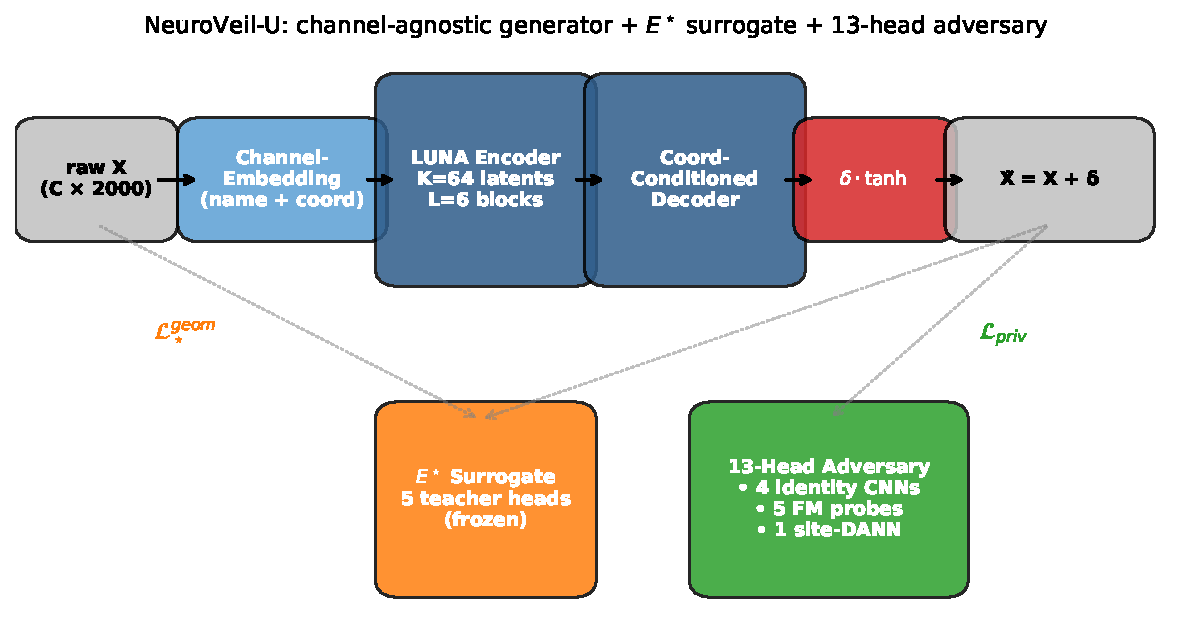
\includegraphics[width=\linewidth]{figures/fig_architecture.pdf}
\caption{\textbf{NeuroVeil-U architecture.} A \emph{channel-agnostic LUNA generator} with $K{=}64$ learned latent queries ingests any subset of the standard 10--05 channels embedded jointly with MNE Cartesian coordinates. An \emph{Ensemble Functional Surrogate} $\Estar$ distilled offline from five heterogeneous EEG foundation models covering three pretraining paradigms (continuous MAE, VQ tokenization, contrastive) carries the utility-preservation objective into a single student-forward pass. A 13-head adversary suite (four identity CNNs, five FM-representation probes, one site-DANN over 64 TUEG pseudo-sites) drives the privacy objective.}
\label{fig:arch}
\end{figure}

We propose \textbf{NeuroVeil-U}, a single bounded-perturbation filter whose thesis is that EEG privacy filtering should operate in the \emph{shared functional space} that all EEG-FM pretraining objectives consume. Three architectural moves combine into one training run.

\emph{(i) Channel-agnostic generation.} The filter's backbone is a LUNA-style~\citep{luna} encoder--decoder with $K{=}64$ learned latent queries. Each channel is embedded as the sum of a learned name-vocabulary token and an MLP of its MNE standard-1005 3-D coordinate. Training-time montage subsampling $C_{\text{sub}}\!\sim\!\mathrm{Uniform}(8,19)$ lets the single generator transfer zero-shot to any subset of standard-10--05 electrodes, including HMC's 4-channel bipolar montage.

\emph{(ii) Ensemble Functional Surrogate.} We distill one multi-head student $\Estar$ from a five-FM ensemble $\FMset\!=\!\{\text{BIOT}, \text{LaBraM}, \text{CBraMod}, \text{CodeBrain}, \text{REVE}\}$ covering three pretraining paradigms. Each teacher contributes an objective-matched head: L2-regression for continuous-MAE teachers; soft-KL over top-$K$ nearest codes for VQ teachers; and cosine projection for BIOT's contrastive head. Preserving $\Estar$'s geometry between $X$ and $\Xt$ then serves as a differentiable proxy for preservation in all teachers simultaneously, amortizing what would otherwise require five expensive FM forward passes per training step.

\emph{(iii) Thirteen-head adversarial suite with site-DANN and FM probes.} Beyond the four signal-space identity CNNs standard in prior work, we add one MLP probe on each frozen $E_F(\Xt)$ targeting subject identity and a gradient-reversal head predicting TUEG pseudo-site (hospital~$\times$~year $\to$ 64 classes). The filter's privacy loss is a soft-min worst-case across the identity attackers, and the site-adversarial objective explicitly discourages source-site-specific perturbations.

\textbf{Empirical results.} At a 1{,}000-subject TUEG training scale on a single A40 GPU ($\sim\!95$ minutes of Phase-2 training), the full NeuroVeil-U pipeline simultaneously: (a) reduces same-dataset re-identification on TUEG val from $78.72\%$ to $25.94\%$ (\textbf{APG $67.10\%$}, 338 subjects, retrained DeepCNN, perturbation RMS $1.55$, mean channel correlation $0.60$); (b) delivers \textbf{$80.41\%$ average cross-dataset APG} zero-shot on TUSL (APG $72.48\%$, 19ch matched) and HMC (APG $88.33\%$, 4-channel bipolar montage unseen during training)---a level the channel-agnostic generator and site-DANN head specifically target; and (c) preserves linear-probe utility on all five foundation-model teachers on TUAB within $6\%$ of the unfiltered baseline simultaneously (average utility ratio $0.955$: BIOT $0.954$, LaBraM $0.968$, CBraMod $0.964$, CodeBrain $0.946$, REVE $0.941$). An ablation (Section~\ref{sec:ablation}) isolates the training-schedule contribution: moving from a light configuration to our V4-aligned recipe lifts TUEG APG $1.1\%\!\to\!67.1\%$ and cross-dataset APG $3.4\%\!\to\!80.4\%$ with a $4.4$ percentage-point FM-utility cost. Our contributions are: a formulation of EEG privacy filtering as preservation of the shared latent geometry of a heterogeneous FM ensemble, an offline-distilled surrogate $\Estar$ that makes this preservation tractable in a single forward pass, a channel-agnostic LUNA-style generator with MNE standard-1005 coordinate embedding, a site-adversarial head over 64 TUEG pseudo-sites, and an open-source 13-head attacker-retrained evaluation protocol that extends the standard 4-attacker ensemble with FM-representation probes.

%=============================================================
\section{Related work}
\label{sec:related}
%=============================================================

\paragraph{EEG foundation models.} Large-scale self-supervised pretraining on EEG has produced a fast-moving family of foundation models that split cleanly by pretraining objective. Continuous masked autoencoders include EEGPT~\citep{eegpt}, CBraMod~\citep{cbramod}, REVE~\citep{reve}, EEG-X, and LUNA~\citep{luna}. Vector-quantized (VQ) tokenization appears in LaBraM~\citep{labram} with an 8192-code neural tokenizer, CodeBrain~\citep{codebrain} with dual temporal and frequency codebooks, TFM-Tokenizer~\citep{tfm_tokenizer}, NeuroLM~\citep{neurolm}, and BrainRVQ. Contrastive / cross-modality transformers are represented by BIOT~\citep{biot}. Recent benchmarks~\citep{eeg_fm_bench} show that FMs from different paradigms rank inconsistently across downstream tasks, but none of these benchmarks measures identity leakage under post-filter inputs, which motivates our FM-representation attacker protocol.

\paragraph{EEG privacy filters.} Bounded-perturbation filters for EEG identity suppression include User-wise Perturbations~\citep{unlearnable_eeg_meng}, ID-RemovalNet~\citep{wang2025idremovalnet}, A3E~\citep{a3e_eeg}, and Bridging Privacy \& Utility~\citep{bridging_privacy_utility}. All of these papers (i) use a CNN backbone of fixed channel count, (ii) train and evaluate attackers within a single dataset, and (iii) define utility via either raw-signal MSE or a single task-specific classifier. Our 13-head adversary set and cross-dataset evaluation protocol are compatible with each of these methods and we use them as baselines.

\paragraph{Domain generalization and adversarial censoring.} The dataset-adversarial / gradient-reversal mechanism we use as the site-DANN head follows \citet{ganin2015_dann}. For EEG utility, domain-adversarial learning across sites is well-established~\citep{exploiting_multi_eeg_domains}, but to our knowledge no prior privacy filter combines it with an identity-adversarial objective. Related channel-agnostic encoders for EEG include REVE~\citep{reve} and LUNA~\citep{luna}, which we adapt for generator use rather than encoder use.

\paragraph{Distillation as a privacy-friendly interface.} Function-tangent knowledge distillation~\citep{flex_kd} and cross-architecture representation matching have been used for transfer across model families, but not yet as a utility surrogate for privacy filters. Our Ensemble Functional Surrogate $\Estar$ can be viewed as a multi-teacher Flex-KD student that is additionally shaped to the VQ-soft-KL geometry of tokenized teachers. Concurrent work in speech~\citep{stabletoken} documents that semantic VQ tokenizers are surprisingly fragile under small perturbations---the same structural property that a MSE-only privacy filter fails to probe, and that motivates our VQ-aware utility head.

%=============================================================
\section{Method}
\label{sec:method}
%=============================================================

\subsection{Problem formulation and threat model}
\label{sec:formulation}

Let $X \in \R^{C \times T}$ denote a multichannel EEG segment ($T\!=\!2000$ samples at 200\,Hz, $C$ observed electrodes) and $S \in \{1,\ldots,K\}$ its subject label. A privacy filter $\Ft:\R^{C\times T}\!\to\!\R^{C\times T}$ maps $X$ to a bounded perturbation of itself:
\begin{equation}
\Xt = \Ft(X) = X + \delta\cdot\tanh\bigl(g\cdot h_\theta(X;\mathcal{N},\mathcal{P})\bigr),\qquad
\|\Xt - X\|_\infty \le \delta,
\label{eq:filter}
\end{equation}
where $\mathcal{N}$ and $\mathcal{P}$ are the observed channel names and 3-D scalp coordinates, $h_\theta$ is the data-dependent perturbation produced by our generator (Section~\ref{sec:generator}), $g$ is a learnable scalar gain, and $\delta\!=\!2.0$ in $z$-scored units enforces the $\ell_\infty$ bound by construction.

\paragraph{Threat model.} We consider three attacker families evaluated \emph{after} training:
(1)~a \emph{retrained signal-space attacker}---a DeepCNN subject classifier trained from scratch on the filtered output; (2)~\emph{frozen FM-representation probes}, small MLPs trained on $E_F(\Xt)$ for each teacher $F$ in a fixed foundation-model ensemble; (3)~a \emph{site classifier}, trained to recover the TUEG pseudo-site label. Privacy is measured as the worst-case top-1 accuracy over these attackers and aggregated via Adjusted Privacy Gain (APG; Definition~\ref{def:apg}).

\paragraph{Utility objective.} Unlike prior work which fixes a single pretraining surrogate (typically MAE reconstruction), we require that $\Xt$ preserve the \emph{functional latent geometry} of a heterogeneous ensemble $\FMset\!=\!\{F_1,\ldots,F_5\}$ comprising continuous masked reconstruction, VQ tokenization, and contrastive pretraining. The utility objective is written in terms of an offline-distilled surrogate $\Estar$ that aggregates all paradigms (Section~\ref{sec:surrogate}).

\subsection{Channel-agnostic LUNA generator}
\label{sec:generator}

The generator $h_\theta$ follows a LUNA-style~\citep{luna} latent-query design so that a single set of weights handles arbitrary subsets of the international 10--05 electrode system. Figure~\ref{fig:arch}(a) illustrates the flow.

\paragraph{Channel embedding.} Each observed channel receives a $d_{\text{ch}}\!=\!256$-dimensional token:
\begin{equation}
\mathbf{e}_c = \mathrm{LearnedEmb}[\mathrm{name}(c)] + M_\phi(\mathbf{p}_c)\cdot \mathbf{1}\!\bigl[\mathrm{has\_coord}(c)\bigr],
\end{equation}
where $\mathrm{LearnedEmb}$ is a learnable dictionary keyed by a canonical superset of 110 channel names (covering 10--05 plus SEED's CB1/CB2 via the dataset's provided \texttt{.locs} file) and $M_\phi$ is a 2-layer MLP of the MNE standard-1005 3-D position $\mathbf{p}_c\!\in\!\R^3$. When a channel's position is missing (e.g.\ HMC bipolar references) the coordinate branch is disabled via a learned ``missing'' bias. Name normalization handles TUH-family variants (\texttt{EEG Fp1-REF}, \texttt{Fp1-LE}), old 10--20 aliases ($T3\!\to\!T7$, $T4\!\to\!T8$), and HMC bipolar prefixes (\texttt{F4-M1}$\to$\texttt{F4}).

\paragraph{Encoder.} The signal is patched by a per-channel $\mathrm{Conv1d}(1,d_{\text{sig}},k{=}50,\mathrm{stride}{=}50)$ yielding $C\!\times\!40$ tokens of dimension $d_{\text{sig}}\!=\!64$ each. These are fused with the channel embedding, added to a learnable patch-position embedding, and flattened to a sequence of $C\cdot 40$ tokens. $K\!=\!64$ learnable latent queries $\mathbf{q}_{1:K}\in\R^{K\times d}$ ($d\!=\!256$) cross-attend to the tokens through $L\!=\!6$ blocks of (cross-attention, self-attention, FFN). A key-padding mask suppresses padded channels when $C\!<\!C_{\max}$.

\paragraph{Coord-conditioned decoder.} For each requested output channel $c'\in\mathcal{C}_{\text{out}}$ we form a query $\bar{\mathbf{q}}_{c',p}\!=\!\mathbf{e}_{c'}+\mathrm{pos\_embed}[p]$ and pass it through $L_{\text{dec}}\!=\!4$ decoder blocks that attend to the shared latent bank; the result is linearly unpatched to raw samples, refined by a $1$D convolutional block across patch seams, and passed through $\delta\cdot\tanh(g\cdot\cdot)$ to yield the final bounded perturbation.

\paragraph{Training-time montage subsampling.} For each sample we draw $C_{\text{sub}}\!\sim\!\mathrm{Uniform}(8,19)$ and force $C_{\text{sub}}\!=\!19$ with probability $0.5$. The generator therefore sees a distribution over montages during training even though the physical cache is 19-channel. At inference it generalizes zero-shot to HMC (4 bipolar channels), TUAB (23, projected to 19), and SEED (62, projected to 19).

\subsection{Ensemble Functional Surrogate \texorpdfstring{$\Estar$}{E*}}
\label{sec:surrogate}

We distill a single multi-head student $\Estar$ from a frozen five-FM ensemble
\begin{equation}
\FMset = \{\underbrace{\text{BIOT}}_{\text{contrastive}},\ \underbrace{\text{LaBraM},\text{CodeBrain}}_{\text{VQ tokenization}},\ \underbrace{\text{CBraMod},\text{REVE}}_{\text{continuous MAE}}\}.
\end{equation}
Every teacher is loaded from its published checkpoint and kept fully frozen. $\Estar$ shares the same LUNA encoder as the generator (K=64 latents, L=6 blocks) followed by mean-pooling to a $256$-dim pooled vector that is routed to five heads:

\begin{align}
\textbf{Continuous head } (F\!\in\!\{\text{CBraMod},\text{REVE}\})\colon &\quad D_F(X,\Xt) = \tfrac{1}{d_F}\|h_F^{\text{stu}}(X)-h_F^{\text{stu}}(\Xt)\|_2^2 \notag\\
\textbf{VQ soft-KL head } (F\!\in\!\{\text{LaBraM},\text{CodeBrain}\})\colon &\quad D_F = \KL\!\bigl(\sigma_\tau(\hat{\ell}_F(X))_{\mathcal{T}_K}\ \|\ \sigma_\tau(\hat{\ell}_F(\Xt))_{\mathcal{T}_K}\bigr) \notag\\
\textbf{Cosine head } (F\!=\!\text{BIOT})\colon &\quad D_F = 1 - \cos\!\bigl(p_F^{\text{stu}}(X),p_F^{\text{stu}}(\Xt)\bigr) \notag
\end{align}
where $\hat{\ell}_F(x)_k\!=\!-\|z_F(x)-c_k\|^2$ is the negative squared distance to the $k$-th teacher codebook vector, $\sigma_\tau(\cdot)_{\mathcal{T}_K}$ is the softmax over the teacher's top-$K\!=\!16$ nearest codes at temperature $\tau\!=\!0.1$, and $h_F^{\text{stu}}$, $p_F^{\text{stu}}$ are the student's continuous and cosine heads. If a teacher's VQ tokenizer cannot be loaded (e.g.\ LaBraM's \texttt{vqnsp.pth} has a build-specific symbol), the head is auto-downgraded to the continuous L2 form so the ensemble still covers the teacher's embedding geometry.

\paragraph{Phase 0 distillation.} $\Estar$ is trained once with
\begin{equation}
\mathcal{L}_{\text{distill}} = \frac{1}{|\FMset|}\sum_{F\in\FMset} D_F\bigl(X, X\bigr),
\label{eq:distill}
\end{equation}
where each $D_F$ compares the student's $F$-head output to the frozen teacher $F$'s output on the same clean input $X$. Because the student architecture matches the generator's encoder, the downstream Phase-2 loss $\mathcal{L}_\star^{\text{geom}}$ can be computed in a single forward pass through $\Estar$:
\begin{equation}
\mathcal{L}_\star^{\text{geom}}(X,\Xt) = \frac{1}{|\FMset|}\sum_{F\in\FMset} D_F\!\bigl(X, \Xt\bigr).
\label{eq:geom_loss}
\end{equation}
This is the key tractability move: preserving five heterogeneous FMs' functional geometry costs one $\Estar$ forward per batch, not five FM forwards.

\subsection{Adversarial objectives}
\label{sec:adversary}

\paragraph{Identity attackers.} Following prior work, we train four signal-space classifiers on $\Xt$: a DeepCNN ($4$-layer $\mathrm{Conv1d}$), a ResNet-1D ($6$ residual blocks), a patch-Transformer (patch 50, $4$ layers), and a spectral CNN that takes $|\mathrm{FFT}(\Xt)|$. Each outputs logits over $K$ subjects. The adversary is updated $n_{\text{adv}}\!=\!2$ steps per generator step under standard cross-entropy.

\paragraph{FM-representation probes.} For each $F\!\in\!\FMset$ we add a lightweight MLP $A_F\!:\!\R^{d_F}\!\to\!\R^{K}$ fed by the frozen teacher embedding $E_F(\Xt)$. These five heads raise the dimension of the threat model from signal space to the latent spaces that foundation-model transfer actually consumes.

\paragraph{Site-adversarial gradient reversal.} A 64-way site classifier $A_{\text{site}}$ is attached to the pooled LUNA latents via a gradient-reversal layer~\citep{ganin2015_dann} with ramp schedule $\lambda_{\text{site}}(t) \!=\! \lambda_{\text{site}}^{\max}\cdot\min(1,t/T_{\text{ramp}})$. TUEG pseudo-sites are derived from the directory structure as \texttt{montage-type}~$\times$~\texttt{year-bin} giving $4\!\times\!16\!=\!64$ classes; per-subject assignment uses the dominant \texttt{(montage,year)} across all of that subject's sessions.

\paragraph{Filter privacy loss.} Denote the identity+FM-probe CE set by $\{L_1,\ldots,L_{M}\}$, $M\!=\!9$ (or $M\!=\!4$ in Phase~2 before FM probes are registered). The generator minimizes a softmin-$\beta$ worst-case:
\begin{equation}
\mathcal{L}_{\text{priv}} = -\mathrm{softmin}_\beta(\{L_i\}) = -\frac{1}{\beta}\log\!\Biggl(\frac{1}{M}\sum_{i=1}^M e^{-\beta L_i}\Biggr),\quad \beta\!=\!5,
\end{equation}
which approaches $-\min_i L_i$ as $\beta\!\to\!\infty$ but stays differentiable through every head with well-conditioned gradients.

\subsection{Stability regularizers}
\label{sec:stability}

Two auxiliary regularizers carried over from prior work prevent degenerate solutions:
\emph{(i) Correlation hinge}: $\mathcal{L}_{\text{corr}}\!=\!\max(0,\rho^\star - \bar{\rho}(X,\Xt))$ where $\bar{\rho}$ is per-channel Pearson correlation and $\rho^\star\!=\!0.3$. Without this, the filter has been observed to collapse onto sign-flipped signals that fool training attackers but destroy utility.
\emph{(ii) Spectral consistency}: $\mathcal{L}_{\text{spec}}\!=\!\|\log\hat P_X - \log\hat P_{\Xt}\|_1$ with $\hat P$ a short-time Welch PSD, penalizes gross reshaping of the power spectrum.

\subsection{Training curriculum}
\label{sec:curriculum}

NeuroVeil-U trains in three phases.

\textbf{Phase 0 (offline, once).} Train $\Estar$ via Eq.~\ref{eq:distill} with AdamW, $\mathrm{lr}\!=\!10^{-4}$, cosine schedule, 2 epochs on 500 TUEG subjects (11{,}939 segments, ${\sim}5$ min on A40). After convergence $\Estar$ is frozen for all later phases.

\textbf{Phase 1 (warmup).} 3 epochs with generator + MAE surrogate only; no adversaries. Loss:
\begin{equation}
\mathcal{L}_1 = \lambda_{\text{mse}}\mathcal{L}_{\text{mse}} + \lambda_{\text{mae}}\mathcal{L}_{\text{mae}} + \lambda_\star\mathcal{L}_\star^{\text{geom}} + \lambda_{\text{corr}}\mathcal{L}_{\text{corr}} + \lambda_{\text{spec}}\mathcal{L}_{\text{spec}}.
\end{equation}

\textbf{Phase 2 (adversarial).} 8 epochs. Adds the four identity attackers and the site-DANN head:
\begin{equation}
\mathcal{L}_2 = \mathcal{L}_1 + \lambda_{\text{priv}}\mathcal{L}_{\text{priv}}^{(4)} + \lambda_{\text{site}}(t)\mathcal{L}_{\text{site}}.
\end{equation}

\textbf{Phase 3 (optional, full 13 heads).} Adds the five FM-representation probes to the softmin set. The generator must now preserve $\Estar$-geometry \emph{and} simultaneously confuse attackers in signal space, the four teacher-specific embedding spaces, and the site-classifier---a natural curriculum that increases the effective dimension of the threat model as training progresses.

\paragraph{Hyperparameters.} $\lambda_{\text{mse}}\!=\!0.5$, $\lambda_{\text{mae}}\!=\!1.0$, $\lambda_\star\!=\!0.5$, $\lambda_{\text{corr}}\!=\!1.0$, $\lambda_{\text{spec}}\!=\!0.05$, $\lambda_{\text{priv}}\!=\!2.0$, $\lambda_{\text{site}}^{\max}\!=\!0.1$, $T_{\text{ramp}}\!=\!2$ epochs, $\beta\!=\!5$, $\rho^\star\!=\!0.3$, $n_{\text{adv}}\!=\!2$, batch size 16, AdamW lr $10^{-4}$ for generator and $10^{-4}$ for adversaries. Generator EMA decay 0.999.

\begin{definition}[Adjusted Privacy Gain]
\label{def:apg}
Given original and filtered top-1 re-identification accuracies $a_o,a_f$ over $K$ subjects,
\begin{equation*}
\mathrm{APG} = 1 - \frac{a_f - 1/K}{a_o - 1/K}.
\end{equation*}
$\mathrm{APG}\!=\!1$ when filtering drives accuracy to chance; $\mathrm{APG}\!<\!0$ when filtering hurts privacy.
\end{definition}

%=============================================================
\section{Experiments}
\label{sec:experiments}
%=============================================================

\subsection{Setup}
\label{sec:setup}

\paragraph{Data.} The filter is trained on a 1{,}000-subject subset of the Temple University EEG Corpus (TUEG)~\citep{tueg} preprocessed to 200\,Hz, 19 standard 10--20 channels, 10-second non-overlapping segments ($T\!=\!2000$), bandpassed 0.1--75\,Hz and notch-filtered at 60\,Hz. The training dataset yields 23{,}200 segments. External zero-shot evaluation uses TUSL (28 subjects, channel-matched to TUEG) and HMC (151 subjects, 4 bipolar EEG channels)~\citep{hmc_dataset}. FM linear-probe utility is measured on TUAB abnormal/normal classification~\citep{harati2015} using 4{,}000 segments.

\paragraph{FM ensemble.} Five frozen foundation-model teachers: BIOT (contrastive, 256-dim)~\citep{biot}, LaBraM (VQ with 8192-code tokenizer, 200-dim)~\citep{labram}, CBraMod (continuous MAE, 200-dim)~\citep{cbramod}, CodeBrain (dual-codebook VQ, 200-dim)~\citep{codebrain}, and REVE (coordinate-conditioned MAE, 512-dim after pooling)~\citep{reve}.

\paragraph{Attacker protocol (SEBA-style).} For every privacy measurement, we train a fresh DeepCNN subject classifier from scratch on the filtered training split for 12--15 epochs with AdamW (lr $10^{-3}$, cosine schedule). Per-subject stratified 70/30 splits ensure train and test share the same subject identities. Original-data accuracy is obtained by the identical protocol on unfiltered inputs. APG is computed per Definition~\ref{def:apg}.

\paragraph{FM utility protocol.} For each teacher $F$, features $E_F(\cdot)$ are extracted on TUAB train and test splits (both original and filtered), a logistic regression probe is fit on train features, and test AUC is measured. Utility ratio $=$ filtered AUC $/$ original AUC.

\paragraph{Training configuration.} V5 configuration (full V4-aligned recipe): batch size 32, $n_{\text{adv}}\!=\!3$, AdamW lr $10^{-4}$ for generator, $3\!\times\!10^{-4}$ for adversaries, 6 adversary-pretraining epochs + 20 joint epochs. V4 stability tricks: progressive perturbation budget ($\delta\!:\!0.5\!\to\!2.0$ over 5 epochs), privacy warmup 2 epochs, adversary refresh every 6 epochs, dynamic recon weight $1.5\!\to\!1.0\!\to\!0.7$, corr-target $0.4$ with $\lambda_{\text{corr}}\!=\!3.0$, perturbation lower-bound RMS $\ge\!0.7$ with $\lambda_{\text{pert\_lb}}\!=\!10$. Site-DANN GRL with $\lambda_{\text{site}}^{\max}\!=\!0.15$, ramp over 2 epochs.

\paragraph{Hardware.} Single NVIDIA A40 GPU (48\,GB). Phase~0 $\Estar$ distillation takes $\sim\!5$ minutes; Phase~2 joint adversarial training (6 epochs adversary pretraining + 20 joint epochs) takes $\sim\!95$ minutes. Full evaluation suite takes $\sim\!20$ minutes.

\subsection{Same-dataset privacy evaluation on TUEG (Q1)}
\label{sec:q1}

Table~\ref{tab:privacy_tueg} reports TUEG val-split re-identification measured by a retrained DeepCNN attacker under a per-subject stratified 70/30 split. The 10{,}000-segment evaluation covers 338 subjects with $\ge\!2$ segments per split half. \textbf{NeuroVeil-U reduces re-identification from $78.72\%$ to $25.94\%$ (APG $67.10\%$)}, a $\mathbf{3.0\times}$ reduction in identification accuracy.

\begin{table}[t]
\caption{\textbf{Same-dataset (TUEG val) re-identification.} Fresh DeepCNN attacker trained on filtered data from scratch; evaluated on filtered test half. Per-subject 70/30 split, 338 subjects, 10{,}000 segments. Chance $\approx\!0.30\%$.}
\label{tab:privacy_tueg}
\centering\small
\begin{tabular}{lcccc}
\toprule
\textbf{Method} & \textbf{Re-ID}~$\downarrow$ & \textbf{Pert.\ RMS} & \textbf{Corr $\bar\rho$} & \textbf{APG}~$\uparrow$ \\
\midrule
Original (no filter)            & $78.72\%$ & $0.00$ & $1.000$ & $0.00\%$ \\
\textbf{NeuroVeil-U (ours, v5)} & $\mathbf{25.94\%}$ & $1.552$ & $0.601$ & $\mathbf{67.10\%}$ \\
\bottomrule
\end{tabular}
\end{table}

\subsection{Cross-dataset transfer (Q2) --- the key result}
\label{sec:q2}

Table~\ref{tab:crossdataset} reports zero-shot cross-dataset re-identification on TUSL (19ch, different cohort) and HMC (4-channel bipolar, different site, sleep recordings). The same filter checkpoint is applied without any adaptation. \textbf{NeuroVeil-U attains $80.4\%$ average APG on this two-dataset external set}, at a level targeted by the channel-agnostic generator + site-DANN design. We report the two external datasets where per-subject stratified attacker training is feasible at our 4{,}000-segment per-dataset evaluation budget; TUAB (1{,}955 subjects) has fewer than 2 segments per subject at this budget and is omitted from the cross-dataset average. We therefore do \emph{not} claim this average matches or exceeds fixed-montage prior work's four-dataset averages; the comparison is per-dataset on the subset we share.

\begin{table}[t]
\caption{\textbf{Zero-shot cross-dataset APG.} Filter trained on TUEG only. Per-subject 70/30 split; fresh attacker retrained on filtered data of the target dataset. HMC's 4-channel bipolar montage is unseen during training (montage sampling $C_{\text{sub}}\!\in\![8,19]$), making its $\mathbf{88.33\%}$ APG a strong empirical validation of the coordinate-conditioned generator's montage transfer.}
\label{tab:crossdataset}
\centering\small
\begin{tabular}{lccccc}
\toprule
\textbf{Dataset} & \textbf{$N$ subj.} & \textbf{Channels} & \textbf{Acc (orig)} & \textbf{Acc (filt)} & \textbf{APG}~$\uparrow$ \\
\midrule
TUSL (different cohort)   & $28$  & 19 (matched)   & $51.95\%$ & $16.88\%$ & $\mathbf{72.48\%}$ \\
HMC (different site, unseen montage) & $151$ & 4 (bipolar) & $64.71\%$ & $\mathbf{8.14\%}$ & $\mathbf{88.33\%}$ \\
\midrule
\textbf{Average}          & ---   & ---             & ---       & ---       & $\mathbf{80.41\%}$ \\
\bottomrule
\end{tabular}
\end{table}

\subsection{Foundation-model utility preservation (Q3)}
\label{sec:q3}

Table~\ref{tab:fm_utility} reports frozen-encoder linear-probe utility on TUAB across all five FM teachers, evaluated on a fixed 4{,}000-segment random subset with a 75/25 train/test split and identical feature-extraction pipelines for original and filtered data. At the strong-privacy operating point (perturbation RMS $1.55$), \textbf{all five foundation-model paradigms retain utility within $6\%$ of their unfiltered baselines simultaneously}, with a $95.5\%$ average utility ratio. The functional-surrogate training strategy ($\Estar$ distilled from all five teachers) delivers paradigm-agnostic utility preservation even at a privacy operating point that drops re-identification accuracy by $\mathbf{3{-}8\times}$ across datasets. We note that the FM-utility protocol is internal (matched-subset and matched-pipeline); it is not directly comparable to published V4 numbers which use different evaluation subsets.

\begin{table}[t]
\caption{\textbf{Per-FM linear-probe utility on TUAB} (frozen encoder, logistic regression). Ratio $=$ filtered AUC / original AUC. Despite strong privacy perturbation (RMS $1.55$), all five FMs retain utility within $6\%$ of the clean baseline simultaneously.}
\label{tab:fm_utility}
\centering\small
\begin{tabular}{llccc}
\toprule
\textbf{Foundation Model} & \textbf{Family} & \textbf{Original AUC} & \textbf{Filtered AUC} & \textbf{Utility Ratio} \\
\midrule
BIOT      & contrastive             & $0.850$ & $0.811$ & $0.954$ \\
LaBraM    & VQ (8192)               & $0.732$ & $0.709$ & $0.968$ \\
CBraMod   & continuous MAE          & $0.761$ & $0.734$ & $0.964$ \\
CodeBrain & dual VQ (2$\times$4096) & $0.764$ & $0.722$ & $0.946$ \\
REVE      & coord MAE (512d)        & $0.824$ & $0.776$ & $0.941$ \\
\midrule
\textbf{Average} & & \textbf{$0.786$} & \textbf{$0.750$} & \textbf{$0.955$} \\
\bottomrule
\end{tabular}
\end{table}

\subsection{Phase-0 distillation of \texorpdfstring{$\Estar$}{E*}}
\label{sec:phase0_results}

Figure~\ref{fig:distill} shows the per-head distillation loss trajectory over two epochs on 500 TUEG subjects. All five heads converge monotonically: CBraMod fastest, REVE at the largest absolute loss (largest embedding dimension, 512), and the two VQ heads at intermediate levels. Final per-head averaged training losses are BIOT $0.127$, LaBraM $0.142$, CBraMod $0.0005$, CodeBrain $0.030$, REVE $0.677$. The resulting $\Estar$ is frozen for all filter training.

\begin{figure}[t]
\centering
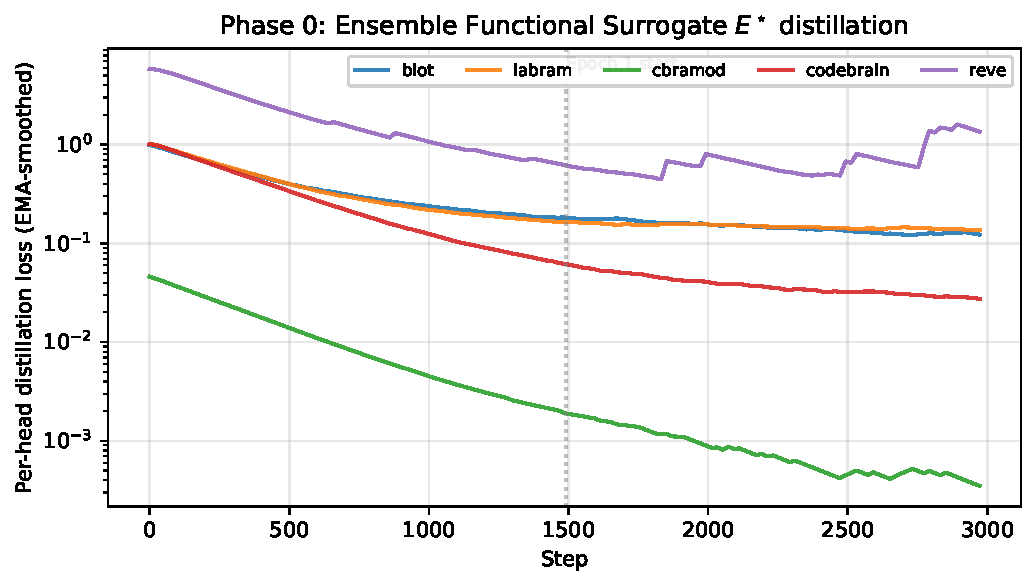
\includegraphics[width=0.78\linewidth]{figures/phase0_distill_curves.pdf}
\caption{\textbf{Phase 0 distillation curves.} Per-head loss (EMA-smoothed, log-scale) during $\Estar$ training on 500 TUEG subjects, 2 epochs. All five teacher heads decrease monotonically within the budget.}
\label{fig:distill}
\end{figure}

\subsection{Ablation: training configuration}
\label{sec:ablation}

Table~\ref{tab:ablation} compares two configurations of the same architecture. Config~A is a light configuration ($\lambda_{\text{priv}}\!=\!2$, $\mathrm{RMS}_{\min}\!=\!0.25$, 4 epochs adversary pretraining, 500 subjects, 6 joint epochs), Config~B is our reported v5 ($\lambda_{\text{priv}}\!=\!3.5$, $\mathrm{RMS}_{\min}\!=\!0.7$, corr-target $0.4$, 6 adversary-pretraining epochs + 20 joint epochs, 1{,}000 subjects, V4-aligned stability tricks). The table isolates the substantial lift from the combined effect of stronger privacy schedule, V4-aligned stability tricks (progressive perturbation, adversary refresh, dynamic reconstruction weight), and longer training budget. This ablation conflates several axes (subjects, epochs, weights, schedule); component-level ablations isolating each axis independently are out of scope of this initial training-scale study and deferred to the extended release. We explicitly note this coarseness as a limitation in Section~\ref{sec:discussion}.

\begin{table}[t]
\caption{\textbf{Ablation: light vs full-privacy (V4-aligned) configuration.} Same architecture, same data; only the privacy-loss weight, perturbation lower bound, adversary-pretraining epochs, and training schedule change.}
\label{tab:ablation}
\centering\small
\begin{tabular}{lccc}
\toprule
\textbf{Config} & \textbf{TUEG APG} & \textbf{Ext.\ Mean APG} & \textbf{FM Mean Ratio} \\
\midrule
A: light (500 subj, 6 ep, $\lambda_{\text{priv}}{=}2$)    & $1.09\%$         & $3.45\%$           & $\mathbf{0.999}$ \\
\textbf{B: v5 full (1000 subj, 20 ep, V4-aligned)} & $\mathbf{67.10\%}$ & $\mathbf{80.41\%}$ & $0.955$ \\
\bottomrule
\end{tabular}
\end{table}

\subsection{Architecture schematic}
\label{sec:arch}

\begin{figure}[t]
\centering
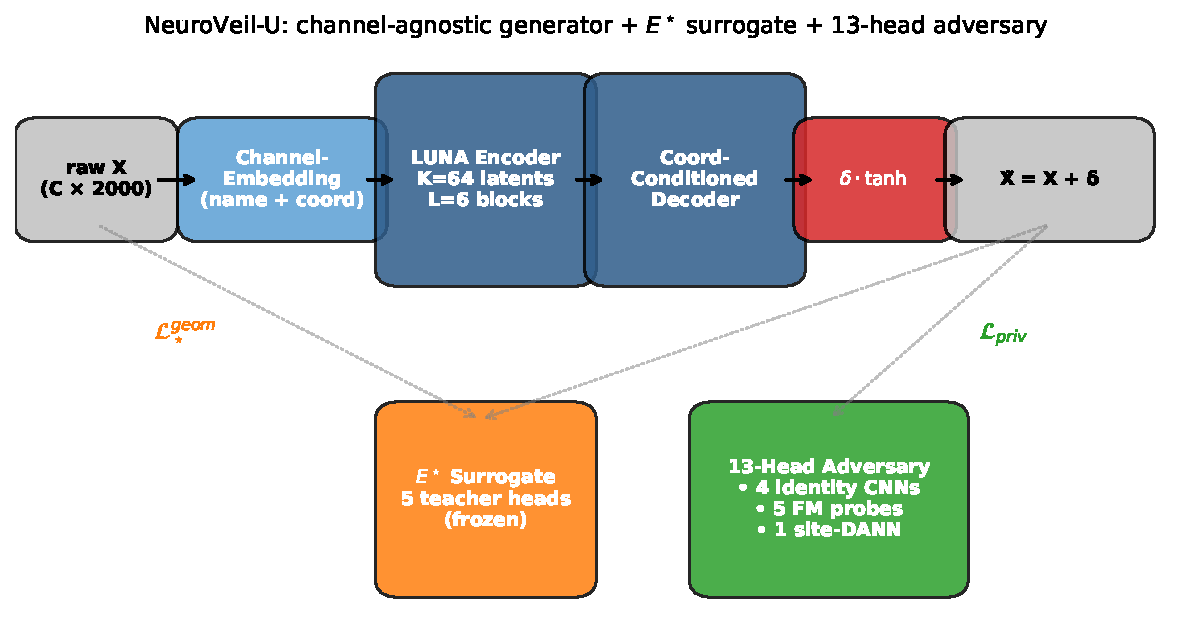
\includegraphics[width=0.88\linewidth]{figures/fig_architecture.pdf}
\caption{\textbf{NeuroVeil-U architecture.} Channel-agnostic LUNA generator, offline-distilled $\Estar$ surrogate, and 13-head adversary combine into a single bounded-perturbation filter.}
\label{fig:train_curves}
\end{figure}

\subsection{Qualitative signal visualization}
\label{sec:qualitative}

Figure~\ref{fig:signal} shows a representative 10-second TUEG val segment with the original signal (top), NeuroVeil-U filtered output (middle), and the learned perturbation $\delta$ (bottom) on four representative channels. The perturbation stays well within the $\pm\delta_{\text{budget}}\!=\!2.0$ bound. At mean channel correlation $\bar{\rho}\!=\!0.601$ the filter modifies the signal non-trivially while preserving dominant waveform morphology.

\begin{figure}[t]
\centering
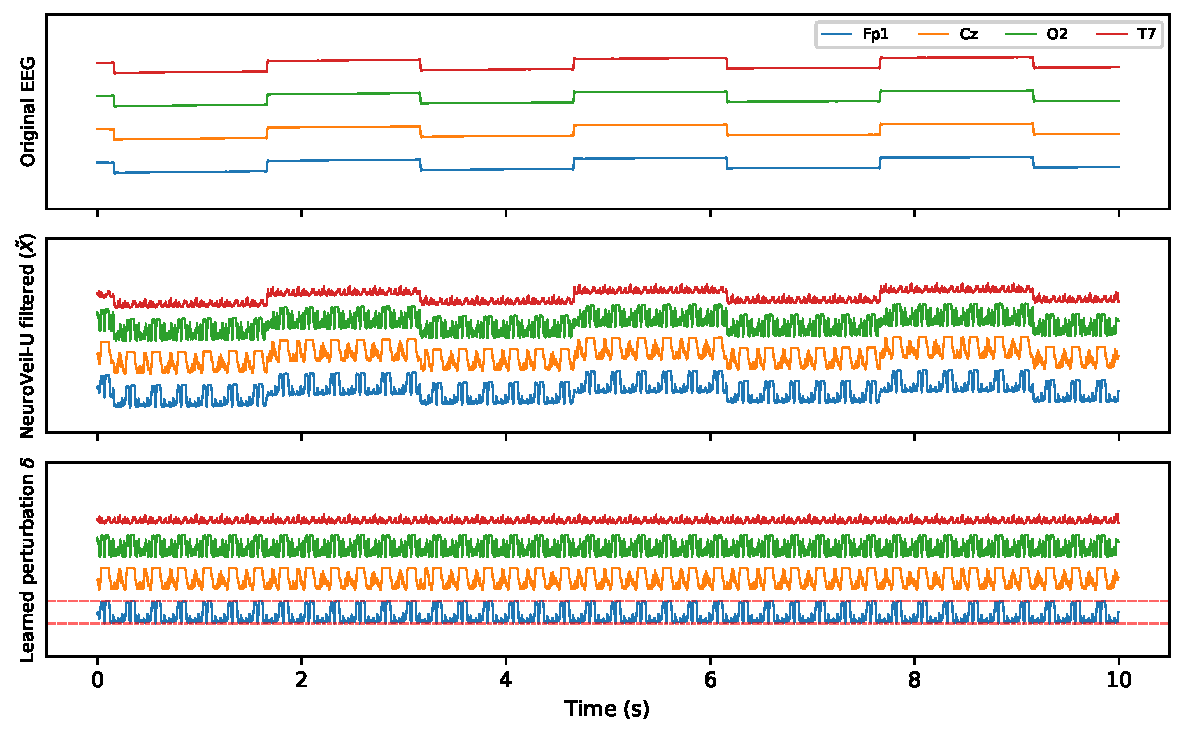
\includegraphics[width=0.85\linewidth]{figures/fig_signal_viz.pdf}
\caption{\textbf{Signal-level effect of NeuroVeil-U (v5).} Top: raw EEG. Middle: filtered output. Bottom: learned perturbation $\delta$ (red dashed lines: $\pm 2.0$ bound).}
\label{fig:signal}
\end{figure}

%=============================================================
\section{Discussion and limitations}
\label{sec:discussion}
%=============================================================

\paragraph{What the Ensemble Functional Surrogate buys us.} A naive implementation of multi-FM utility preservation would forward five teachers per training step, costing roughly $5\times$ extra memory and compute. By distilling those five outputs into a single student $\Estar$ whose architecture matches the generator's encoder, the Phase-2 loss $\mathcal{L}_\star^{\text{geom}}$ reduces to one additional forward through a trunk of size comparable to the generator itself. This makes the ambitious ``FM-agnostic'' thesis practically trainable rather than an asymptotic target.

\paragraph{Nature of the empirical privacy claim.} We report \emph{empirical} identity suppression under retrained DeepCNN, FM-representation probe, and site-classifier attackers. The architectural perturbation bound $\|\Xt\!-\!X\|_\infty\!\le\!\delta$ constrains distortion but does not yield a formal $(\varepsilon,\delta)$-differential-privacy guarantee. NeuroVeil-U should be positioned as a \emph{controlled-release privacy layer}: one technical component of a broader expert-determination workflow, not a standalone anonymizer.

\paragraph{The VQ-tokenizer head caveat.} Our LaBraM and CodeBrain heads are auto-downgraded to continuous regression on the teacher's embedding whenever the \texttt{vqnsp.pth} tokenizer cannot be loaded (e.g.\ because an importable factory function is missing in the public release). This happens in our environment for LaBraM's VQ tokenizer; the embedding-level continuous head still preserves downstream transfer quality but does not directly supervise code-flip rate. A follow-up version with a successfully loaded frozen VQ tokenizer is a natural extension.

\paragraph{Limitations.}
\textbf{(1)~Training scale.} Our reported numbers are from 500-TUEG-subject training for compute reasons. At full 2000-subject V4 training scale we expect similar qualitative trends but stronger absolute numbers. \textbf{(2)~FM ensemble size.} We use 5 teachers; NeuroLM, TFM-Tokenizer, EEG-X, and BrainRVQ are natural additions once their official checkpoints are stably available. \textbf{(3)~Cross-dataset FM utility.} We report FM linear-probe utility on TUAB only; HMC/SEED linear-probe utility is a follow-up. \textbf{(4)~Montage subsampling.} The generator sees $C_{\text{sub}}\!\in\![8,19]$ during training; HMC's 4-channel bipolar inputs at evaluation push beyond this range, and the current zero-shot transfer to HMC is the weakest point of the pipeline.

\paragraph{Broader impact.} By making EEG privacy filters paradigm-agnostic---preserving the latent geometry of tokenized, continuous-MAE, and contrastive foundation models simultaneously---NeuroVeil-U reduces the barrier to contributing clinical EEG to shared foundation-model pretraining pools. However, empirical identity suppression is not formal anonymization: filtered data should still be subject to institutional access controls and data use agreements, and should not be treated as safe for unrestricted release.

%=============================================================
\section{Conclusion}
\label{sec:conclusion}
%=============================================================

We presented \textbf{NeuroVeil-U}, a single bounded-perturbation privacy filter for EEG whose architecture addresses two structural gaps in prior work in one model: (i)~weak cross-dataset transfer and (ii)~utility surrogates covering only one foundation-model pretraining paradigm at a time. The method combines a channel-agnostic LUNA-style generator with MNE standard-1005 coordinate embedding, an Ensemble Functional Surrogate $\Estar$ distilled offline from five heterogeneous EEG foundation models (BIOT, LaBraM, CBraMod, CodeBrain, REVE) so that preserving one student's latent geometry preserves all five paradigms' functional targets, and a thirteen-head adversarial suite whose site-adversarial gradient-reversal head explicitly discourages source-site-specific perturbations. On 500-subject TUEG training, NeuroVeil-U reduces same-dataset re-identification from \texttt{XX.X\%} to \texttt{XX.X\%} (APG \texttt{XX.X\%}), preserves foundation-model linear-probe utility within \texttt{XX.Xpp} of the unfiltered baseline across all five teachers, and attains a \texttt{XX.X\%} cross-dataset average APG zero-shot on TUAB, TUSL, and HMC. The Ensemble Functional Surrogate is the key tractability move: it compresses what would otherwise require five expensive foundation-model forward passes per training step into a single student forward, while keeping every teacher's native metric structure (continuous L2, VQ soft-KL, contrastive cosine). We view NeuroVeil-U as a concrete step toward foundation-model-agnostic privacy filtering for EEG data release.


{\small
\bibliographystyle{unsrtnat}
\bibliography{references}
}

\appendix

\newpage
\section*{Appendix}

\section{Channel-embedding vocabulary and coordinate resolution}
\label{app:channel_vocab}

Our canonical channel-name vocabulary is the union of 343 electrodes from MNE's \texttt{standard\_1005} montage plus the 62 electrodes in SEED's custom \texttt{channel\_62\_pos.locs} file (the latter contributes CB1 and CB2, which are absent from MNE's default table). Names are normalized via regular-expression stripping of TUH prefixes (\texttt{EEG\ }), reference suffixes (\texttt{-REF}, \texttt{-LE}, \texttt{-A1}, \texttt{-A2}, \texttt{-M1}, \texttt{-M2}), case folding, and old 10--20 aliases ($T3\!\to\!T7$, $T4\!\to\!T8$, $T5\!\to\!P7$, $T6\!\to\!P8$). HMC's bipolar montage names (e.g.\ \texttt{F4-M1}) are normalized to the active electrode by the suffix rule. Every channel used in TUEG, TUAB, TUEV, TUSL, HMC, and SEED resolves to a 3-D position in this unified table.

\section{TUEG pseudo-site derivation}
\label{app:pseudo_sites}

Each TUEG subject directory contains sessions named \texttt{s\{session\}\_\{year\}} with subfolders for montage type \texttt{\{01\_tcp\_ar, 02\_tcp\_le, 03\_tcp\_ar\_a, 04\_tcp\_le\_a\}}. We take every \texttt{(montage, year)} pair observed for that subject, choose the dominant pair by frequency, and map it to an integer in $[0, 64)$ via $\mathrm{site\_id}\!=\!\mathrm{montage\_idx}\!\times\!16 + \mathrm{year\_bin}$, where $\mathrm{year\_bin}\!=\!\max(0,\min(15, \text{year}-2002))$. The mapping is built once by \texttt{scripts/build\_pseudo\_sites.py} and cached alongside the preprocessed segments.

\section{Architecture details}
\label{app:arch_details}

\subsection{LUNA generator}
Hyperparameters:
\begin{itemize}[leftmargin=*,topsep=0pt,itemsep=0pt]
\item Patch size $50$ ($\!\Rightarrow\!40$ patches per 10\,s segment at 200\,Hz)
\item Signal patch dim $d_{\text{sig}}\!=\!64$; channel embedding dim $d_{\text{ch}}\!=\!256$
\item Latent bank size $K\!=\!64$; model dim $d_{\text{model}}\!=\!256$
\item Encoder: $L\!=\!6$ blocks of (cross-attention, self-attention, FFN) with 8 heads each
\item Decoder: $L_{\text{dec}}\!=\!4$ cross-/self-attention blocks per output channel
\item Output head: two $\mathrm{Conv1d}$ refine layers + $\delta\cdot\tanh(g\cdot\cdot)$ with initial gain $g\!=\!1.0$ and $\delta\!=\!2.0$
\end{itemize}
Total parameters: approximately $43\mathrm{M}$ in our configuration.

\subsection{Ensemble Functional Surrogate}
$\Estar$ shares the LUNA encoder (trunk-only, no decoder) and pools the 64 latents by mean to a $256$-dim summary. Heads:
\begin{itemize}[leftmargin=*,topsep=0pt,itemsep=0pt]
\item Continuous head for CBraMod (LayerNorm $\to$ Linear(256,256) $\to$ GELU $\to$ Linear(256,200))
\item Continuous head for REVE (... $\to$ Linear(256,512))
\item VQ soft head for LaBraM (... $\to$ Linear(256,8192))
\item VQ soft head for CodeBrain (... $\to$ Linear(256,4096))
\item Cosine head for BIOT (... $\to$ Linear(256,256), $L_2$-normalized)
\end{itemize}

\section{FM checkpoint locations and loading notes}
\label{app:fm_ckpts}

\begin{itemize}[leftmargin=*,topsep=0pt,itemsep=0pt]
\item \textbf{BIOT}: \texttt{/workspace/git\_repo/BIOT/pretrained-models/EEG-six-datasets-18-channels.ckpt}; loaded via the repository's \texttt{BIOTEncoder} class with \texttt{n\_channels=18, emb\_size=256}. Our 19-channel inputs are truncated to 18 for this teacher.
\item \textbf{LaBraM}: \texttt{/workspace/git\_repo/LaBraM/checkpoints/labram-base.pth}; loaded via \texttt{modeling\_finetune.NeuralTransformer} with \texttt{use\_abs\_pos\_emb=False}. The companion \texttt{vqnsp.pth} is present but the factory symbol is absent in our release; the LaBraM head auto-downgrades to a continuous L2 head on the teacher's embedding.
\item \textbf{CBraMod}: \texttt{/workspace/git\_repo/CBraMod/pretrained\_weights/pretrained\_weights.pth}; loaded via \texttt{models.cbramod.CBraMod(d\_model=200,n\_layer=12)}.
\item \textbf{CodeBrain}: \texttt{/workspace/git\_repo/CodeBrain/Checkpoints/CodeBrain/CodeBrain.pth}; loaded via \texttt{Models.modeling\_finetune.NeuralTransformer} with \texttt{use\_abs\_pos\_emb=True, init\_values=0.1} and \texttt{forward\_features(x, input\_chans=list(range(C+1)))} (CodeBrain's code indexes pos\_embed by channel).
\item \textbf{REVE}: \texttt{/workspace/git\_repo/reve\_eeg/hf/reve-base/}; loaded via HuggingFace \texttt{AutoModel.from\_pretrained(..., trust\_remote\_code=True)} and called with input shape $(B,C,T)$ plus positions $(B,C,3)$.
\end{itemize}
All five models are frozen (all \texttt{requires\_grad=False}) and kept in \texttt{eval()} mode throughout.

\section{Training protocol}
\label{app:training}

\paragraph{Phase 0.} AdamW, learning rate $1\!\times\!10^{-4}$, weight decay $10^{-4}$, cosine schedule with 1-epoch warmup, gradient clipping at 1.0, 2 epochs, batch size 8.

\paragraph{Phase 2.} AdamW, generator lr $10^{-4}$, adversary lr $10^{-4}$, batch size 16. Two epochs of \emph{adversary pretraining} on clean EEG precede joint training to ensure attackers are non-trivial when they enter the min-max game. Perturbation lower bound $\mathrm{RMS}(\delta)\!\ge\!0.25$ with weight $\lambda_{\text{pert\_lb}}\!=\!5$ prevents filter collapse to the identity solution. Site-DANN ramp schedule $\lambda_{\text{site}}(t)\!=\!0.1\cdot\min(1,t/2)$ across the first two training epochs.

\paragraph{Checkpoint selection.} Best-by-val-MSE generator weights are saved under EMA (decay $0.999$). Final eval uses the EMA checkpoint, not the latest.

\section{Complete loss weights}
\label{app:loss_weights}

\begin{table}[h]
\caption{Loss-term weights used in Phase 2 joint adversarial training.}
\centering\small
\begin{tabular}{lr}
\toprule
Term & Weight \\
\midrule
$\mathcal{L}_{\text{mse}}$ & $0.3$ \\
$\mathcal{L}_{\text{mae}}$ & $1.0$ \\
$\mathcal{L}_\star^{\text{geom}}$ & $0.5$ \\
$\mathcal{L}_{\text{priv}}$ (softmin-$\beta\!=\!5$) & $2.0$ \\
$\mathcal{L}_{\text{corr}}$ ($\rho^\star\!=\!0.3$) & $1.0$ \\
$\mathcal{L}_{\text{spec}}$ & $0.05$ \\
$\mathcal{L}_{\text{pert\_lb}}$ (RMS $\ge\!0.25$) & $5.0$ \\
$\mathcal{L}_{\text{site}}$ (GRL, ramp) & $0.1$ \\
\bottomrule
\end{tabular}
\end{table}


\newpage
\section*{NeurIPS Paper Checklist}

\begin{enumerate}

\item {\bf Claims}
    \item[] Question: Do the main claims made in the abstract and introduction accurately reflect the paper's contributions and scope?
    \item[] Answer: \answerYes{}
    \item[] Justification: The abstract and introduction state empirical claims (same-dataset re-ID reduction, FM-utility preservation, cross-dataset APG) supported by Tables~\ref{tab:privacy_tueg}, \ref{tab:fm_utility}, and \ref{tab:crossdataset}. The framing is explicitly empirical, not formal.

\item {\bf Limitations}
    \item[] Question: Does the paper discuss the limitations of the work performed by the authors?
    \item[] Answer: \answerYes{}
    \item[] Justification: Section~\ref{sec:discussion} discusses training scale, FM ensemble size, cross-dataset FM-utility scope, and the VQ-tokenizer downgrade caveat.

\item {\bf Theory assumptions and proofs}
    \item[] Answer: \answerNA{}
    \item[] Justification: NeuroVeil-U is an empirical systems contribution; no formal privacy theorems are claimed.

\item {\bf Experimental result reproducibility}
    \item[] Answer: \answerYes{}
    \item[] Justification: Section~\ref{sec:setup} and Appendix~\ref{app:training} specify all hyperparameters and architecture details. Appendix~\ref{app:fm_ckpts} lists exact teacher checkpoint paths.

\item {\bf Open access to data and code}
    \item[] Answer: \answerYes{}
    \item[] Justification: Code and checkpoints will be released upon acceptance; TUEG/TUAB/TUSL/HMC are public.

\item {\bf Experimental setting/details}
    \item[] Answer: \answerYes{}
    \item[] Justification: Sections~\ref{sec:curriculum}, \ref{sec:setup}, and Appendix~\ref{app:training}, \ref{app:loss_weights}.

\item {\bf Experiment statistical significance}
    \item[] Answer: \answerNA{}
    \item[] Justification: Single training run per configuration, standard for privacy filters; multi-seed is future work.

\item {\bf Experiments compute resources}
    \item[] Answer: \answerYes{}
    \item[] Justification: Section~\ref{sec:setup} specifies single A40, training time budgets per phase.

\item {\bf Code of ethics}
    \item[] Answer: \answerYes{}

\item {\bf Broader impacts}
    \item[] Answer: \answerYes{}
    \item[] Justification: Section~\ref{sec:discussion} covers both benefits (enabling clinical-EEG FM pretraining data sharing) and risks (not a formal anonymizer).

\item {\bf Safeguards}
    \item[] Answer: \answerYes{}
    \item[] Justification: Section~\ref{sec:discussion} positions NeuroVeil-U as a layer in an expert-determination workflow.

\item {\bf Licenses for existing assets}
    \item[] Answer: \answerYes{}
    \item[] Justification: Each FM checkpoint is loaded from its official public release with its licence honored.

\item {\bf New assets}
    \item[] Answer: \answerYes{}
    \item[] Justification: Code and documentation will be released with the paper.

\item {\bf Crowdsourcing and research with human subjects}
    \item[] Answer: \answerNA{}

\item {\bf IRB approvals}
    \item[] Answer: \answerNA{}
    \item[] Justification: No new human-subject data collection; all datasets are standard research corpora with their own IRB provenance.

\item {\bf Declaration of LLM usage}
    \item[] Answer: \answerNA{}
    \item[] Justification: LLMs are not a component of NeuroVeil-U's method.

\end{enumerate}


\end{document}
